\documentclass[11pt]{article}
%\usepackage[version=3]{mhchem} % Package for chemical equation typesetting
%\usepackage{siunitx} % Provides the \SI{}{} and \si{} command for typesetting SI units
%\usepackage{graphicx} % Required for the inclusion of images
%\usepackage{natbib} % Required to change bibliography style to APA
\usepackage{amsmath} % Required for some math elements 
\usepackage[margin=1in]{geometry}
\usepackage{microtype}
\usepackage[english]{babel}
\usepackage[utf8]{inputenx}
\usepackage{float}
\usepackage{graphics}
\usepackage{graphicx}
\usepackage{subfigure}
\usepackage{amsmath}
\usepackage{textcomp}
\usepackage{makeidx}
\usepackage{hyperref}
\usepackage{braket}
%\usepackage[latin1]{inputenc}
\usepackage{amsthm}
\usepackage{amsfonts}
\usepackage{amssymb}
\usepackage{graphicx}
\usepackage{fullpage}
\usepackage{hyphenat}
\usepackage{float}
\usepackage{longtable}
\usepackage{picture}
\usepackage{multicol}
\usepackage{fancyhdr}
\usepackage{wrapfig}
\usepackage{geometry}

\theoremstyle{theorem}
\newtheorem{theorem}{Theorem}
\newtheorem{proposition}{Proposition}

\theoremstyle{definition}
\newtheorem{definition}{Definition}



%\usepackage{tikz}
%\usetikzlibrary{graphs}
%\usepackage{pgfplots}
%\pgfplotsset{compat=newest}

\setlength\parindent{0pt} % Removes all indentation from paragraphs

\renewcommand{\figurename}{Grafico}
\renewcommand{\tablename}{Tabella}
\newcommand{\at}[2][]{#1\Big|_{#2}}
\renewcommand{\labelenumi}{\alph{enumi}.} % Make numbering in the enumerate environment by letter rather than number (e.g. section 6)

%\usepackage{times} % Uncomment to use the Times New Roman font

%----------------------------------------------------------------------------------------
%	DOCUMENT INFORMATION
%----------------------------------------------------------------------------------------

\title{C1 - Assignment 1 Report: Sparse Matrices.} % Title

\author{Student Number: 1894945} % Author name

\date{\today} % Date for the report

\begin{document}

\maketitle % Insert the title, author and date

\begin{center}
C1 - Assignment 1 Report \hfill
Student Number: 1894945
\vspace{3pt} \hrule \vspace{3pt} \hrule
\end{center}

%\clearpage
\tableofcontents

\clearpage
% If you wish to include an abstract, uncomment the lines below
%\begin{abstract}


%\end{abstract}
%\clearpage 

\section{Introduction}

\subsection{Well-posed, direct problems}
The problems that have been addressed in the present assignment are always representable in the form: 

\begin{equation}
	\label{eqn:general-problem}
	F(x, d) = 0
\end{equation}

where $x$ represents the unknown, $d$ the set of data from which the solution depends on and $F$ the functional relation between $x$ and $d$. Such types of problem are called \emph{direct problems} (\cite{numerical-math}).\\

\begin{definition}
	\label{defn:cont-dep}
	Let $D$ be the set of admissible data, i.e. the set of data for which problem \eqref{eqn:general-problem} admits a unique solution $x$. Let $d\in D$ and denote by $\delta d$ a perturbation such that $d + \delta d\in D$ and by $\delta x$ the corresponding change in the solution, in such a way that:
	
	$$F(d+\delta d, x+\delta x) = 0$$
	
	Then the solution $x$ depends continuously on the data $d$ if
	
	$$\exists\eta_0(d),\hspace{1mm}\exists K_0(d)$$ 
	
	such that:
	
	$$||\delta d||\le\eta_0(d)\implies ||\delta x||\le K_0(d)||\delta d||$$
	 
\end{definition}

If is $x$ continuously dependent on the data $d$, then the problem is said to be \emph{well-posed} or \emph{stable}. Whenever such a property is not satisfied, the problem is said to be \emph{ill-posed}.\\

\subsection{Numerical Methods}
In the following, it will always be assumed that problem \eqref{eqn:general-problem} is well-posed. A numerical method for problem $\eqref{eqn:general-problem}$ consists in a sequence of approximate problems:

\begin{equation}
	\label{eqn:num-method}
	F_n(x_n, d_n) = 0 \hspace{3mm} n\ge 1
\end{equation}

with the underlying expectation that $x_n\rightarrow x$ as $n\rightarrow\infty$, i.e. the approximate solution converges to the exact one. 

\begin{definition}
	\label{defn:stability}
	Consider the problem 
	
	$$F_n(x_n, d_n)=0, \hspace{3mm} n\in\mathbb{N}$$
	
	and denote $D_n$ the set of admissible data for this problem. Then, the numerical method $F_n$ is stable if its solution $x_n$ depends continuously on the the data $d_n$, for all admissible data $d_n\in D_n$.
\end{definition}

\begin{definition}
	\label{defn:convergence}
The numerical method \eqref{eqn:num-method} is convergent iff

$$\forall\epsilon >0,\hspace{1mm} \exists n_\epsilon,\hspace{1mm} \exists\delta(n_\epsilon)\hspace{3mm} | \hspace{3mm}\forall n > n_\epsilon,\hspace{1mm} \forall\delta d_n : ||x(d)-x_n(d+\delta d_n)||<\epsilon$$

where $\delta d_n$ a perturbation of $d_n$, $d_n$ is an admissible datum for the $n^{th}$ approximate problem,  $x_n(d+\delta d_n)$ the corresponding solution of it and $x(d)$ the solution of the exact problem.
\end{definition}

\subsection{Linear systems}
Consider the following linear system:

$$Ax=b$$

where $A\in\mathbb{R}^{n\times n}$, $x\in\mathbb{R}^n$ and $b\in\mathbb{R}^n$. It is evident that such a problem can be expressed in the form \eqref{eqn:general-problem} as follows:

$$F(x,(A,b))=0$$ 

In order to obtain the solution $x$ of the given problem, one should generally invert $A$ (assuming $A$ is non-singular). One gets:

$$x=A^{-1}b$$ 

The standard \emph{direct} method for inverting a generic dense matrix is given by computing its LU decomposition (see \cite{lec-notes}). The general computational cost for such a procedure is $\mathcal{O}(n^3)$, so that the method becomes impractical if $A$ is large or sparse, as it happens in the present assignment.\\
A naive implementation of a direct method to invert a sparse matrix is a computational waste, both in memory and compute time. One would rather neither store the zeros in a sparse matrix, nor multiply by them. Certainly, a direct method can be adapted to do neither of these things, leading to the \emph{sparse direct methods}. Alternatively, one can rely on the so called \emph{iterative methods}. Iterative methods are a class of matrix inversion techniques depending only on the calculation of matrix–vector multiplications, which are typically relatively easy to implement in the case of sparse matrices (see \cite{lec-notes}).\\
The performance of an iterative method is generally evaluated by the number of iterations required to converge to a sufficiently accurate approximation of the actual solution. A generic sparse-matrix–vector multiplication costs $\mathcal{O}(kn)$ , $k$ being the average number of non-zero elements in each row. Hence, ideally, one desires an iterative method whose computational cost is either independent of $n$ or scales sublinearly with respect to $n$, in order to be competitive with direct methods without relying on the sparsity of the matrix.\\

\subsubsection{Splitting Methods}
\label{subsubsec:splitting-methods}
In order to implement an iterative method, it is necessary to generate a sequence of approximations $\lbrace x^{(k)}\rbrace$ to the solution. In the case of a splitting method for the problem $Ax=b$, the sequence is obtained as follows:

$$Px^{(k+1)}=Nx^{(k)}+b$$

or, equivalently:

$$x^{(k+1)}=x^{(k)}+P^{-1}r^{(k)}$$

where $A=P-N$ is the \emph{splitting matrix}, $P$ is the preconditioner matrix and $r^{(k)}=b-Ax^{(k)}$. In particular, the inversion of
P, which has to be non singular, has not to cost more than $\mathcal{O}(n^2)$ operations, so that the whole method consists in $\mathcal{O}(n^2)$ operations  (the left multiply with N is always this much).\\

\subsubsection{Gauss-Seidel Method}
\label{subsubsec:gauss-seidel-method}
Let the decomposition of $A$ be redefined as $A=D-(E+F)$, where $D$ is the diagonal of $A$, $-E$ and $-F$ are the upper-triangular and lower-triangular components of $A-D$.\\
The Gauss-Seidel method is defined by setting $P_G=D-E$ and $N_G=F$. Clearly, inverting $P_G$ costs $\mathcal{O}(n^2)$.\\
It can be proven (see \cite{lec-notes}, \cite{hac94}) that, if $A\in\mathbb{R}^{n\times n}$ is symmetric and positive definite, then the Gauss-Seidel method converges for any $x^{(0)}$.\footnote{Clearly, in order to improve convergence of the algorithm, an optimal choice of the \emph{initial guess} $x^{(0)}$ can to be made.} As a matter of fact, the convergence of the iterations depends on $\rho(P^{-1}N)$, $\rho(B)$ being the spectral radius of the matrix $B$. More precisely one can show the following to hold true: 

\begin{theorem}
For $b\in\mathbb{R}^n$ and $A=P-N\in\mathbb{R}^{n\times n}$, if P is non-singular and $\rho(P^{-1}N)<1$, then the iterates of the splitting scheme $Px^{(k+1)}=Nx^{(k)}+b$ converge to $x=A^{-1}b$ for any $x^{(0)}$.
\end{theorem}
\begin{proof}
Let $e^{(k)}=x^{(k)}-x$ be the error at the $k^{th}$ iterate. Since $P(x^{(k+1)}-x)=N(x^{(k)}-x)$ one has:

$$e^{(k+1)}=(P^{-1}N)^ke^{(0)}$$

which concludes the proof.
\end{proof}

Taking advantage of the triangular form of $P$, the updating of the $i^{th}$ component of $x$ at the $(k+1)^{th}$ iteration can be written in the following form:
\begin{equation}
	\label{eqn:Gauss-Seidel}
	x_i^{(k+1)}=\frac{1}{a_{ii}}\left[b_i-\sum_{j=1}^{i-1}a_{ij}x_j^{(k+1)}-\sum_{j=i+1}^{n}a_{ij}x_j^{(k)}\right]\hspace{3mm} i=1,\cdots, n
\end{equation}

Hence, in the Gauss-Seidel method, at the $(k+1)^{th}$ step, the available values of $x^{(k+1)}$ are used to update the solution.\\
The algorithm is terminated on the residual $r^{(k)}$, meaning that the iterations stop when

$$||r^{(k)}||<TOL$$

TOL being some error tolerance. It is, however, not clear with respect to which norm the previous condition has to be satisfied: even though the choice a norm is completely subjective, $L_\infty$ and $L_2$ norms are the ones most commonly used (see \cite{lec-notes}). In the following, the $L_\infty$ one will be used.\\

\section{Implementation}
The program has been built with the aim to minimise the memory used to store the matrices. Hence, following the instructions given in the assignment, the STL container \emph{vector} has been used to store both the matrix entries and the corresponding column indexes. However, instead of using simple vectors, vectors of pointers have been used. Such a solution provides a more efficient storing of both entries and indexes, as it can be directly seen by comparing the memory allocated by the program with the case in which simple vectors are used.\\
The initialisation of an instance SparseMatrix is implemented in the following way: the constructor builds two vectors of vectors of pointers, setting the length of the first containers to the size of the matrix, but not initialising the content of the nested containers and setting the size of the rows and columns of the matrix. When a value and an index need to be stored, the \emph{addEntry} function is called and if the row at which the value has to be inserted is non-existing, it is dynamically created: both the value and the index are pushed in. If the row exists already, a simple push$\_$back is performed.\\ 


\subsection{Construction of the Gauss-Seidel function}
The core of the whole program is clearly represented by the function performing the Gauss-Seidel algorithm. Such a function has been chosen to be a member function and has been built to accept 7 parameters: the initial guess $x_0$, the vector to invert against $b$, the tolerance required by the method (\emph{tol}), the number of iterations after which a check for stagnation has to be made (\emph{itCheck}), two files on which the residual error at every iteration and the solution are printed respectively, the maximum number of iteration the user is willing to wait for the algorithm to converge (\emph{MaxIter}).\\
Looking at Eqn. \eqref{eqn:Gauss-Seidel}, it is clear that the elements of $x_0$ can be overwritten as they are computed in the algorithm and only one storage vector is needed: $x_0$ has then been passed by reference to the function, so that no copy of it has to be produced.\\
It is worth pointing out that the matrix entries needed for overwriting the elements of $x_0$ are obtained through the member function $getValue$.\footnote{More comments on this choice can be found in $\S\ref{subsec:perf}$}.\\  
In case the matrix is not a square matrix and the sizes of $x_0$ and $b$ do not equal the row and column size of the matrix, the program exits with an appropriate warning to the user. If this is not the case, the iterations start. The program runs until either the residual error becomes smaller than the given tolerance or the maximum number of iterations \emph{MaxIter} has been reached. In order to make sure that the program has not stagnated, every \emph{itCheck} iterations, the current residual error, in the $L_\infty$ norm, is compared with the one computed and stored \emph{itCheck} iterations before: if the residual has not decreased, the program exits with an appropriate stagnation warning to the user. An appropriate warning is printed on the terminal if the program exist due to having reached the maximum number of iterations the user has fixed.\\
The sudo code for the implementation of the algorithm can be found either in Ref.\cite{lec-notes} or on Wikipedia and will not be reported here. 

\subsection{Testing correctness}
In order to check the correctness of the implementation of the Gauss-Seidel algorithm, the tests requested by the assignment have been performed: for this reason, a non-member function Gauss$\_$Seidel$\_$test has been built. Such a function takes 6 arguments: the size of the matrix $A$ that has to be initialised to perform the test, the parameters $\delta$ and $\lambda$ necessary to the implementation of the same tests, the fixed tolerance (\emph{tol}), the number of iterations after which a check for stagnation has to be made (\emph{itCheck}), the maximum number of iteration the user is willing to wait for the algorithm to converge (\emph{MaxIter}). The last 3 parameters will be used by the member function Gauss$\_$Seidel previously introduced, within the function Gauss$\_$Seidel$\_$test.\\
The vectors $x_0$, $b$, $\omega$ and $D$ and the parameter $a=4(\delta-1)$ necessary to construct the matrix $A$ are initialised by this function. The entries of $A$ are added by means of the member function \emph{addEntry}.\\
The files on which the residual error at every iteration and the corresponding final solution are printed, are identified by the value of $\delta$, the value of $\lambda$, by the strings \emph{Residual} or \emph{solution} and the size of the matrix with on the output files.\\
The function prints on the terminal the error between the exact and the found solution, indexing it through the value of $\lambda$, $\delta$ and the size $N$ of matrix $A$.\\

\subsection{Running the program}
The program is run through the Makefile provided. The current optimisation is set to -Ofast and all following tests have been performed with this optimisation choice. Every possible error or warning has been explicitly checked by means of the instruction \emph{-Wall -Wfatal-errors -pedantic} (that can still be found commented out in the Makefile) before proceeding to performing the different tests: no warnings appeared.\\
The program generates a fixed number of output files, in which the results of the tests have been stored. Some of these files are used to produce plots by means of two different plotscripts.\\


\subsection{Results of the tests}
In the following, the results of the more significant tests performed will be reported and briefly discussed. The tolerance has been set to $10^{-6}$ for each of the tests.

\subsubsection{Varying the matrix size}
The Gauss$\_$Seidel$\_$test function has been shown to work for the case of $N=100$, $N=1000$ and $N=10000$, N being the size of the matrix, as required by the assignment.
The time $T_{10000}$ required to reach convergence in the case $N=10000$ has been explicitly computed trough the following instructions:

\begin{verbatim}
	auto start = std::chrono::high_resolution_clock::now();
	
	auto finish = std::chrono::high_resolution_clock::now();
	std::chrono::duration<double> elapsed = finish - start;
	std::cout<< "Elapsed time: " << elapsed.count() << "s\n";
\end{verbatim} 

and found to be $T_{10000}\approx 83$ seconds. The algorithm has thus been shown to work in quite a short time, so that the program can be regarded as being reasonably efficient.\footnote{More comments on the efficiency of the code can be found in $\S\ref{subsec:perf}$.} The solutions $x_0$ obtained for the three different cases can be found in the files \emph{d$\_$1.000000$\_$l$\_$0.000000$\_$GSsolution$\_$100.txt}, \emph{d$\_$1.000000$\_$l$\_$0.000000$\_$GSsolution$\_$1000.txt} and \emph{d$\_$1.000000$\_$l$\_$0.000000$\_$GSsolution$\_$10000.txt}. The residual error at every iteration has been printed in corresponding \emph{Residual} files.\\
Finally, the distance between the exact solution and the approximate one is printed on the terminal. Unsurprisingly, the error becomes bigger as the size of the matrix grows.\\

\subsubsection{Varying $\delta$}
The performance of the algorithm has been tested for different values of $\delta$, as required by the assignment. Having shown that the algorithm converges in a reasonably short time even in the case of $N=10000$, the size of the matrix for this series of tests has been fixed to $N=100$.\\
In order to investigate the change in performance for different order of magnitudes, 10 different values of $\delta$, ranging from $1.0$ to $10^5$ have been used.

\begin{figure}[H]
	\begin{center}
		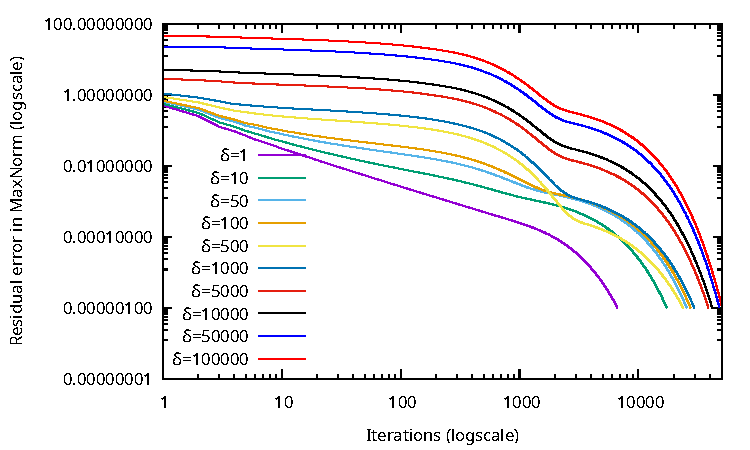
\includegraphics[width=1.0\textwidth]{Gauss_Seidel_delta}
	\end{center}
	\caption{Graphical representation of the performance of the algorithm for different values of $\delta$. To point out the differences between the the results at different orders of magnitude, both the iterations and the residual error in the $L_\infty$ norm have been plotted on a logarithmic scale.
		\label{fig:delta}}
\end{figure} 

It is clear that the desired closeness to the exact solution, measured in terms of the residual error, is reached independently of how large the initial residual is. This is not surprising: in $\S\ref{subsubsec:gauss-seidel-method}$ it has been pointed out that for symmetric and positive definite matrices the method converges for every initial guess $x_0$. As expected, the residual error is a monotone decreasing function of the iterations.\\
For $\delta\ge50$, a concave region in the residual error profile is noticeable, signalling a change in the $``$velocity$"$ of convergence. Interestingly, such a region is particularly steep for $\delta=500$ and an overlap with the curves associated with smaller $\delta$ is present.\\

Clearly, the number of iterations required to have a residual error smaller than the fixed tolerance grows with $\delta$, i.e. the code becomes less efficient when $\delta$ grows. In other words, the spectral radius of the matrix $P^{-1}N$ (see $\S\ref{subsubsec:gauss-seidel-method}$) gets smaller for increasing $\delta$.\\

\subsubsection{Varying $\lambda$}
The performance of the algorithm has been tested for different values of $\lambda$, as required by the assignment. Having shown that the algorithm converges in a reasonably short time even in the case of $N=10000$, the size of the matrix for this series of tests has been fixed to $N=100$.\\
In order to investigate the change in performance for different order of magnitudes, 10 different values of $\lambda$, ranging from $1.0$ to $10^5$ have been used.

\begin{figure}[H]
	\begin{center}
		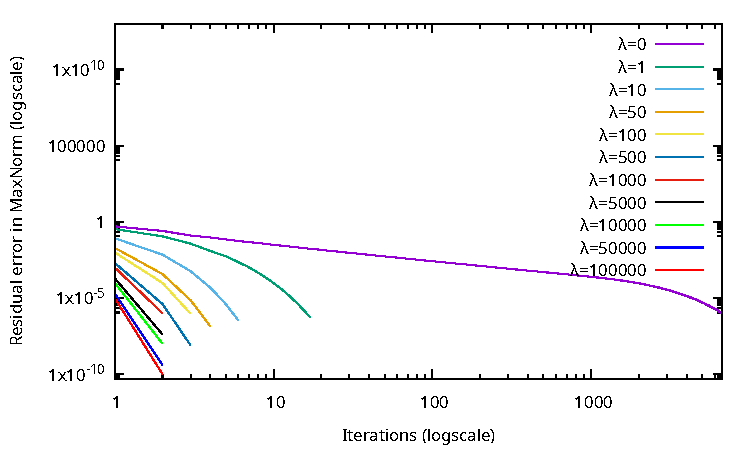
\includegraphics[width=1.0\textwidth]{Gauss_Seidel_lambda}
	\end{center}
	\caption{Graphical representation of the performance of the algorithm for different values of $\lambda$. To point out the differences between the the results at different orders of magnitude, both the iterations and the residual error in the $L_\infty$ norm have been plotted on a logarithmic scale.
		\label{fig:lambda}}
\end{figure} 

It is clear that the presence of $\lambda$ changes the efficiency of the algorithm. In particular, the plot shows that for $\lambda\ge10^3$, the desired convergence is reached in just two iterations.\\
This can be understood by recalling what has been mentioned in $\S\ref{subsubsec:splitting-methods}$ and $\S\ref{subsubsec:gauss-seidel-method}$ about the decomposition of A into $P_G=D-E$ and $N_G=F$. The presence of $\lambda\in\mathbb{R}^{+}$ modifies the diagonal component of $A$ and consequently the matrix $D$. The preconditioner matrix $P$ thereby obtained is different from the one of the initial problem and this results in a faster convergence of the method. As a matter of fact, for $\lambda\in\mathbb{R}^{+}$ the matrix becomes strictly diagonal dominant. Differently from the case of $\delta$, the spectral radius of $P^{-1}N$ becomes smaller and a faster convergence is obtained.\\





\section{Conclusive remarks}
In this section some additional comments and observation are presented.

\subsection{Memory}
When dynamically allocating memory, one has always to make sure to free the reserved locations as soon as they are no longer needed. With the help of the software \emph{valgrind}, possible memory leaks have been checked. To do this, is it necessary to compile with \emph{-g} and \emph{-O1} optimisation. After having compiled the program, the following instruction has been used:

\begin{verbatim}
$ valgrind --leak-check=yes ./sparsematrix
\end{verbatim}

The following output has been produced on the terminal:

\begin{verbatim}
==4200== Memcheck, a memory error detector
==4200== Copyright (C) 2002-2017, and GNU GPL'd, by Julian Seward et al.
==4200== Using Valgrind-3.13.0 and LibVEX; rerun with -h for copyright info
==4200== Command: ./sparsematrix
==4200== 
==4200== 
==4200== HEAP SUMMARY:
==4200==     in use at exit: 0 bytes in 0 blocks
==4200==   total heap usage: 1,252,428 allocs, 1,252,428 frees, 989,616,540 bytes allocated
==4200== 
==4200== All heap blocks were freed -- no leaks are possible
==4200== 
==4200== For counts of detected and suppressed errors, rerun with: -v
==4200== ERROR SUMMARY: 0 errors from 0 contexts (suppressed: 0 from 0)
\end{verbatim}

One can clearly see that no memory has been lost, so that everything has been deleted correctly. \\
It may seem a little strange at fist that all the heap blocks were freed, even though no explicit call to the destructor has been made. However, all instances are built by the function Gauss$\_$Seidel$\_$test, so that the deletion is automatically performed every time the programs exits the function.\\
The absence of memory leaks is however non trivial, since it proves that the destructor has been constructed correctly. This can be explicitly checked by means of commenting out the last two lines of the destructor: if \emph{valgrind} is called again, some memory leak will be found.\\ 


\subsection{Performances}
\label{subsec:perf}
In order to test performance, the following instructions have been used\footnote{The test has been performed only on the part of the code concerned with the test over different $\lambda$ and $\delta$, commenting out the part on different $N$ in the main file. }:
\begin{verbatim}
$ valgrind --tool=callgrind ./sparsematrix
$ kcachegrind
\end{verbatim}

The first command analyses the perfomances in the terms of load distrubution, while \emph{kcachegrind} is used to visualise the load distribution results. Results are reported in the following screenshot.

\begin{figure}[H]
	\begin{center}
		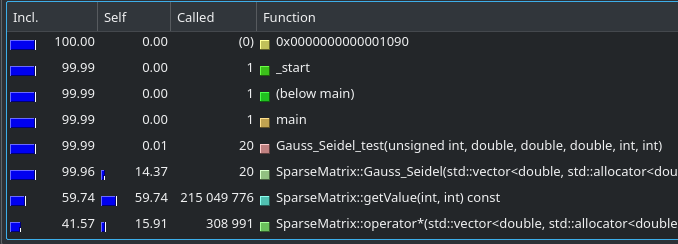
\includegraphics[width=1.0\textwidth]{kcache_perf}
	\end{center}
	\caption{Load distribution of the program.
		\label{fig:load-distr}}
\end{figure} 

It is clear that a better efficiency could have been obtained if the program had not relied so much on the \emph{getValue} function, which is not particularly efficient.\\

\subsubsection{Possible solutions}
A possible way to optimise the code is to sort the indexes and values as soon as they are entered, so that each index can be associated to the corresponding value in a unique way and without the necessity to call a the \emph{getValue}. Such a solution, however, has not been implemented, since even though it is clearly more efficient for the matrix given in the assignment, it is not immediately clear how faster and optimised the code could become in the case of denser sparse matrix. On the other hand, it is still reasonable to expect that such a choice will make the program faster, since the sorting takes place only at the beginning of the program and \emph{getValue} is called a large number of times during the iterations.\\
Possibly, the best solution is to store the values and the indexes by means of the \emph{insert} function instead that through a \emph{push$\_$back}: this way, the values
 will be automatically sorted.\\



\cleardoublepage
%\add1contentsline{toc}{chapter}{\bibname}
\begin{thebibliography}{99}

\bibitem{numerical-math} A. Quateroni, R. Sacco, F. Saleri;
\emph{Numerical Mathematics}, Vol.37, Springer Verlag, (2007).

\bibitem{lec-notes} T. Grafke;
\emph{Scientific Computing}, Lecture Notes, University of Warwick, (2018).

\bibitem{hac94} W. Hackbush; 
\emph{Iterative Solution of Large Sparse Systems of Equations}, Springer-Verlag, New York, (1994).







\printindex
\end{thebibliography}
\bibliography{bibliography} % BibTeX database without .bib extension
\end{document}



%----------------------------------------------------------------------------------------
%	BIBLIOGRAPHY
%----------------------------------------------------------------------------------------

%\bibliographystyle{apalike}

%\bibliography{sample}

----------------------------------------------------------------------------------------


%end{document}